\documentclass[11pt,a4paper]{article}
\usepackage[T1]{fontenc}
\usepackage{lmodern}
\usepackage{amsmath,amssymb}
\usepackage{siunitx}
\usepackage{geometry}
\usepackage{graphicx}
\usepackage{booktabs}
\usepackage{hyperref}
\geometry{margin=2.5cm}

\title{03\_Drag\_Calculation: Coastdown-Based Estimation of CdA and Cr}
\author{Validation\_Aero\_Test}
\date{\today}

\begin{document}
\maketitle

\section{Overview}
This document describes the drag and rolling-resistance estimation from
extracted coastdown runs.  The implementation is split between the shared
library \texttt{aero\_validation/drag.py} and three standalone CLI approach
scripts under \texttt{Code/03\_Drag\_Calculation/}.

\paragraph{Pipeline flow}
\begin{center}
\begin{verbatim}
drag_intervals.csv  +  run_XXX.csv  (from 02_Run_Extraction)
    |
    v
prepare_run_slice()  -->  v, v^2, decel  per run
    |
    v
robust_linear_fit()  -->  k2, c  per run/config
    |
    v
derive_drag_metrics()  -->  CdA, Cr, Fd
    |
    v
summarize_by_config()  -->  per-config stats + wing contributions
\end{verbatim}
\end{center}

\paragraph{Provenance.}
The results shown are from the Stei\ss{}lingen aero-validation test day
(2025-10-22), 4 stints, 46 extracted coastdown runs across 4 aerodynamic
configurations.

\section{Inputs}
\begin{itemize}
  \item Intervals: \texttt{Outputs/02\_Run\_Extraction/csv/drag\_intervals.csv}
        (from the run extraction step; see \texttt{02\_Run\_Extraction.pdf})
  \item Per-run time series: \texttt{Outputs/02\_Run\_Extraction/csv/run\_\{XXX\}.csv}
  \item Vehicle + analysis constants: \texttt{Data/vehicle\_constants.json}
\end{itemize}

The following columns from the cleaned dataset (see \texttt{01\_Data\_Preparation.pdf}) are required in each per-run CSV:
\begin{itemize}
  \item \texttt{t\_s} [s]
  \item \texttt{GPS1\_VEL\_MAG\_ms} [\si{\meter\per\second}]
  \item \texttt{IMU\_ACCEL\_LONG\_ms2} [\si{\meter\per\second\squared}]
\end{itemize}

\section{Reproducibility}
Run the following commands from the repository root after completing the
data-preparation and run-extraction steps:

\begin{verbatim}
# Approach 1: per-run regression
python Code/03_Drag_Calculation/Approach1_PerRun/run.py

# Approach 2: paired opposite-direction averaging
python Code/03_Drag_Calculation/Approach2_PairedOpposites/run.py

# Approach 3: one pooled fit per configuration
python Code/03_Drag_Calculation/Approach3_PooledByConfig/run.py

# Optional: regenerate bootstrap uncertainty estimates
python Code/03_Drag_Calculation/bootstrap_pooled_uncertainty_from_runs.py
\end{verbatim}

All thresholds (minimum speed, filter gates) and the vehicle constants JSON
path can be overridden via CLI arguments of each approach.

\section{Preprocessing per interval}
Preprocessing is implemented in \texttt{aero\_validation/drag.py} as
\texttt{prepare\_run\_slice}.  Given a per-run CSV and an interval $[t_0,t_1]$:
\begin{enumerate}
  \item Slice to \(t\in[t_0,t_1]\).
  \item (Best effort) enforce coastdown conditions if available:
    throttle \texttt{ICU\_Apps\_pct} $\le 1\%$, brakes $\le 0.1$\,bar.
  \item Discard low-speed samples: \(v \ge v_\mathrm{min}\) (default \SI{5}{m/s}).
  \item Define positive deceleration as \(a_\mathrm{dec} = -\,a_\mathrm{long}\).
  \item Smooth \(a_\mathrm{dec}\) with a centered rolling median (default window 7 samples).
  \item Construct regression features \(v\) and \(v^2\).
\end{enumerate}

\section{Model, fitting, and conversions}
\subsection*{Coastdown model}
Neglecting grade and wind, the coastdown dynamics can be approximated by
\[
  m\,\dot v = -\tfrac{1}{2}\,\rho\,C_dA\,v^2 - C_r\,m\,g.
\]
Using the positive deceleration convention \(a_\mathrm{dec}=-\dot v\), the pipeline fits
\[
  a_\mathrm{dec}(v) = k_2 v^2 + c.
\]
The conversions from regression coefficients to physical parameters are:
\[
  C_dA = \frac{2 m k_2}{\rho}, \qquad C_r = \frac{c}{g}.
\]
If a frontal area $A$ is provided per configuration, then
\[
  C_d = \frac{C_dA}{A}.
\]

For reference, the drag and rolling-resistance forces at a given speed $v$ are
\[
  F_d(v) = \tfrac{1}{2}\,\rho\,C_dA\,v^2, \qquad
  F_{rr} = C_r\,m\,g,
\]
so that $m\,a_\mathrm{dec}(v) = F_d(v) + F_{rr}$.

\subsection*{Robust regression}
Two robust fitting helpers (in \texttt{aero\_validation/drag.py}) are used:
\begin{itemize}
  \item \texttt{robust\_linear\_fit}: iterative $2\sigma$ clipping for the 1D model \(y=m x + b\).
  \item \texttt{robust\_linear\_fit\_multi}: iterative $2\sigma$ clipping for a multivariate linear model \(y=X\beta\).
\end{itemize}
Both perform an initial least-squares fit, compute residuals, remove outliers
exceeding a $2\sigma$ threshold ($\sigma$ = standard deviation of residuals),
and refit for up to 5 iterations.  If fewer than 10 points remain after any
iteration, fitting stops and the last valid coefficients are returned.

\subsection*{Vehicle constants and configuration mapping}
Constants are loaded from \texttt{Data/vehicle\_constants.json} via
\texttt{load\_constants} (defined in \texttt{aero\_validation/drag.py}), which
returns a \texttt{VehicleConstants} dataclass.  Missing fields emit a
\texttt{UserWarning} and use sensible defaults, except
\texttt{config\_ranges\_by\_run\_id} which is required and raises a
\texttt{ValueError} if absent.

Key fields:
\begin{itemize}
  \item \texttt{vehicle.mass\_kg}, \texttt{vehicle.rho\_kgm3}
  \item \texttt{vehicle.frontal\_area\_m2\_by\_config} (optional, for reporting \(C_d\))
  \item \texttt{analysis.fd\_speeds\_ms} (reference speeds for drag force table)
  \item \texttt{analysis.baseline\_config} (reference configuration for \(\Delta C_dA\) and wing contributions)
  \item \texttt{analysis.config\_ranges\_by\_run\_id} mapping config name $\rightarrow$ \([\texttt{start},\texttt{end}]\)
\end{itemize}

\subsection*{Wing contribution decomposition}
The aerodynamic configurations are designed to isolate individual wing elements:
\begin{center}
\begin{tabular}{ll}
\texttt{full}           & Both wings installed \\
\texttt{no\_rear}       & Rear wing removed \\
\texttt{no\_front\_rear} & Both wings removed (baseline) \\
\texttt{no\_front}      & Front wing removed \\
\end{tabular}
\end{center}

Wing contributions are computed by differencing the per-configuration mean
$C_dA$ against the baseline:
\begin{align*}
  C_dA_\text{front\_wing} &= C_dA_\text{no\_rear} - C_dA_\text{baseline}, \\
  C_dA_\text{rear\_wing}  &= C_dA_\text{no\_front} - C_dA_\text{baseline}, \\
  C_dA_\text{both\_wings} &= C_dA_\text{full} - C_dA_\text{baseline}.
\end{align*}
These are written to \texttt{drag\_config\_summary\_contributions.csv} by each
approach and reported in the results section below.

\section{Implemented approaches (with example plots)}
Each approach is a standalone CLI script that writes a self-contained output
folder under \texttt{Outputs/03\_Drag\_Calculation/}.

\subsection{Approach 1: Per-run (baseline)}
\texttt{Code/03\_Drag\_Calculation/Approach1\_PerRun/run.py}
\begin{itemize}
  \item Fit \(a_\mathrm{dec}=k_2 v^2 + c\) per extracted interval.
  \item Convert \(k_2,c\) to \(C_dA\) and \(C_r\), then summarize per configuration.
  \item Emit per-run fit plots for QC.
\end{itemize}

\begin{figure}[h]
  \centering
  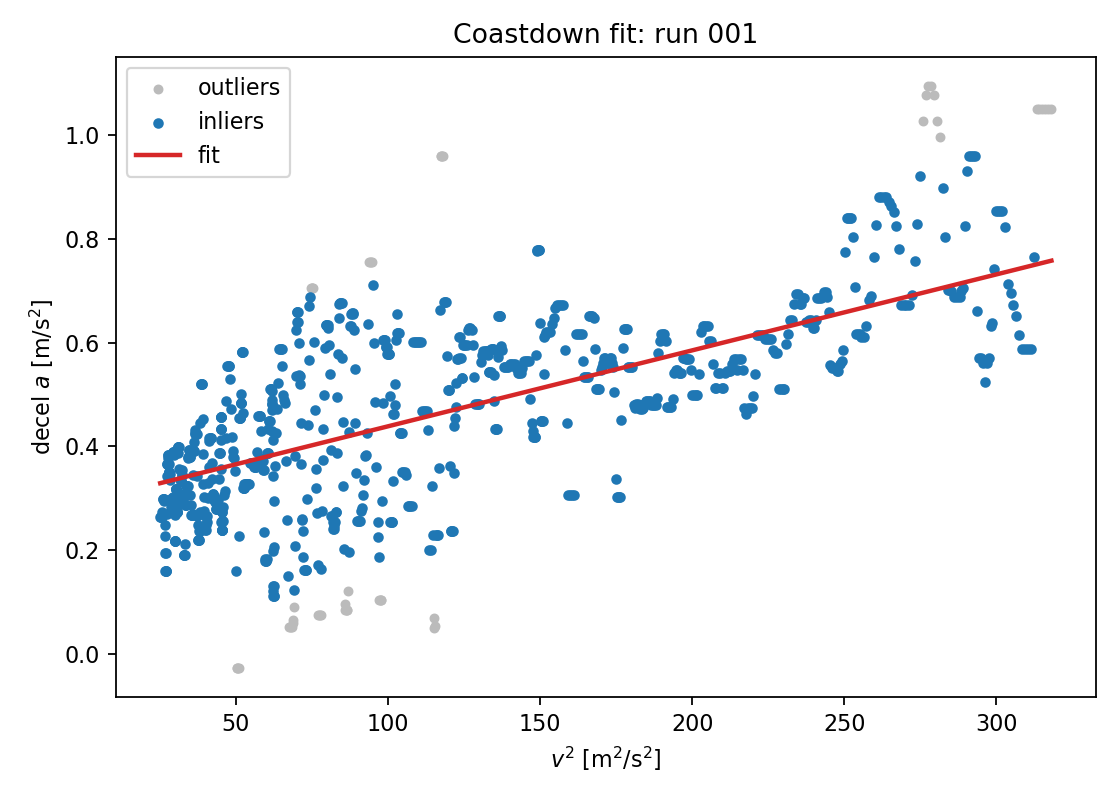
\includegraphics[width=\linewidth]{../../Outputs/03_Drag_Calculation/Approach1_PerRun/plots/coastdown_run_001.png}
  \caption{Approach 1: example per-run coastdown fit plot (Run~001).}
\end{figure}

\begin{figure}[h]
  \centering
  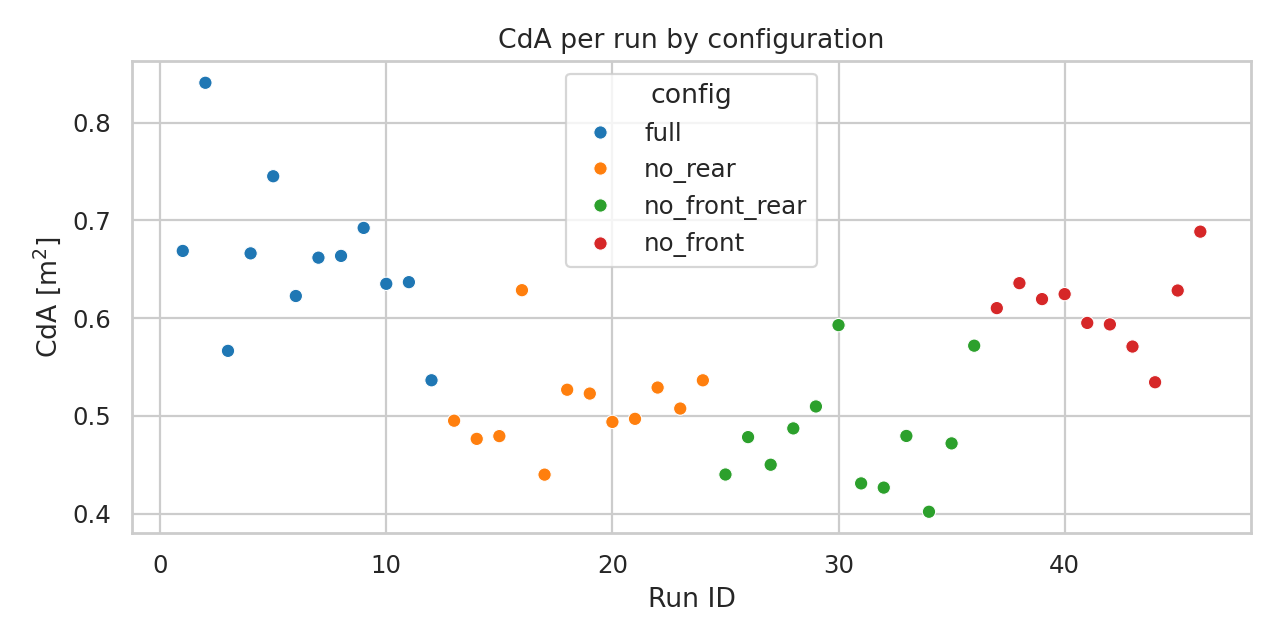
\includegraphics[width=0.95\linewidth]{../../Outputs/03_Drag_Calculation/Approach1_PerRun/plots/CdA_per_run_by_config.png}
  \caption{Approach 1: per-run \(C_dA\) values grouped by configuration.}
\end{figure}

\begin{figure}[h]
  \centering
  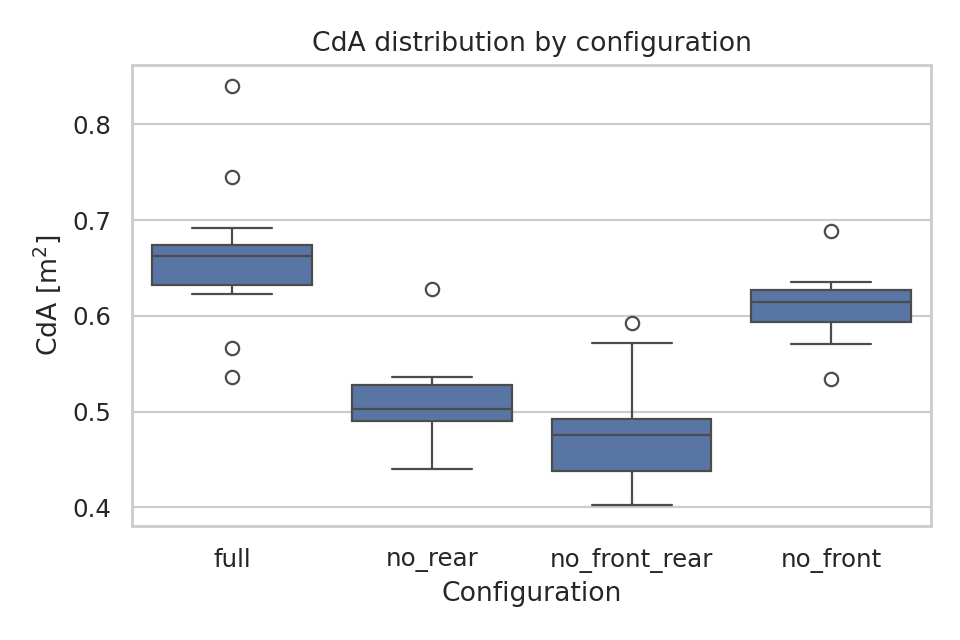
\includegraphics[width=0.85\linewidth]{../../Outputs/03_Drag_Calculation/Approach1_PerRun/plots/CdA_box_by_config.png}
  \caption{Approach 1: \(C_dA\) distribution per configuration (box plot).}
\end{figure}

\subsection{Approach 2: Paired opposites (baseline)}
\texttt{Code/03\_Drag\_Calculation/Approach2\_PairedOpposites/run.py}
\begin{itemize}
  \item Fit per run (as in Approach 1).
  \item Pair consecutive run IDs \((i,i{+}1)\) within a configuration and average coefficients.
  \item Motivation: reduce steady biases that change sign with direction (e.g., wind/grade) when the experiment is executed as out-and-back passes.
\end{itemize}

\begin{figure}[h]
  \centering
  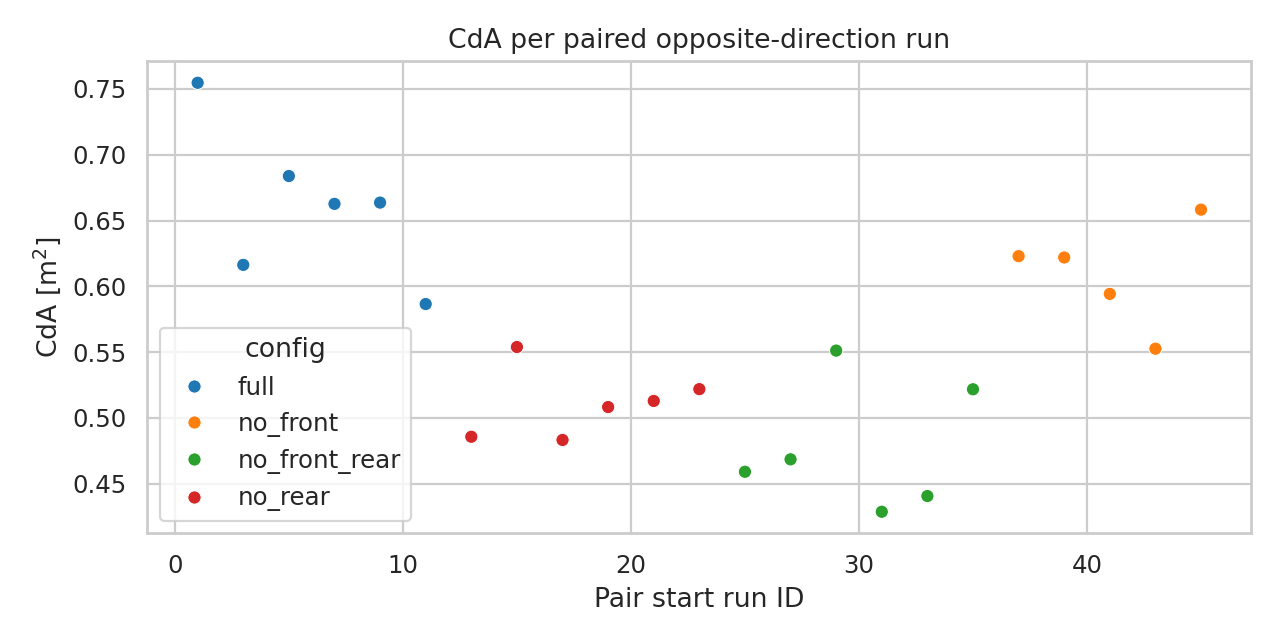
\includegraphics[width=0.95\linewidth]{../../Outputs/03_Drag_Calculation/Approach2_PairedOpposites/plots/CdA_per_pair_by_config.png}
  \caption{Approach 2: \(C_dA\) per paired runs, grouped by configuration.}
\end{figure}

\begin{figure}[h]
  \centering
  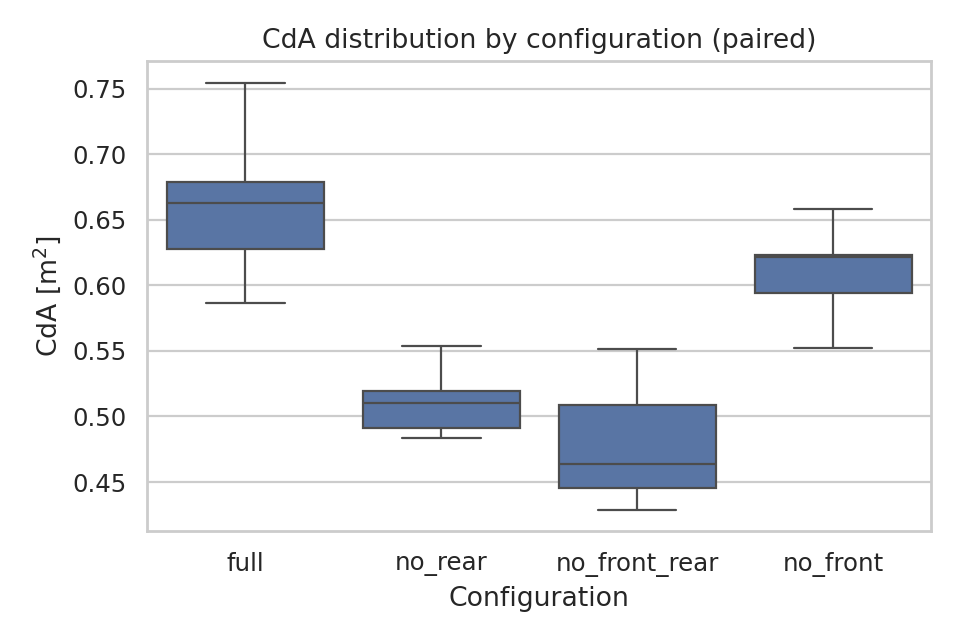
\includegraphics[width=0.85\linewidth]{../../Outputs/03_Drag_Calculation/Approach2_PairedOpposites/plots/CdA_box_by_config_paired.png}
  \caption{Approach 2: \(C_dA\) distribution per configuration after pairing.}
\end{figure}

\subsection{Approach 3: Pooled by configuration (baseline)}
\texttt{Code/03\_Drag\_Calculation/Approach3\_PooledByConfig/run.py}
\begin{itemize}
  \item Stack all samples of all runs belonging to a configuration.
  \item Fit one \(k_2,c\) per configuration using robust regression.
  \item Motivation: maximize point count and reduce sensitivity to short noisy runs.
\end{itemize}

\begin{figure}[h]
  \centering
  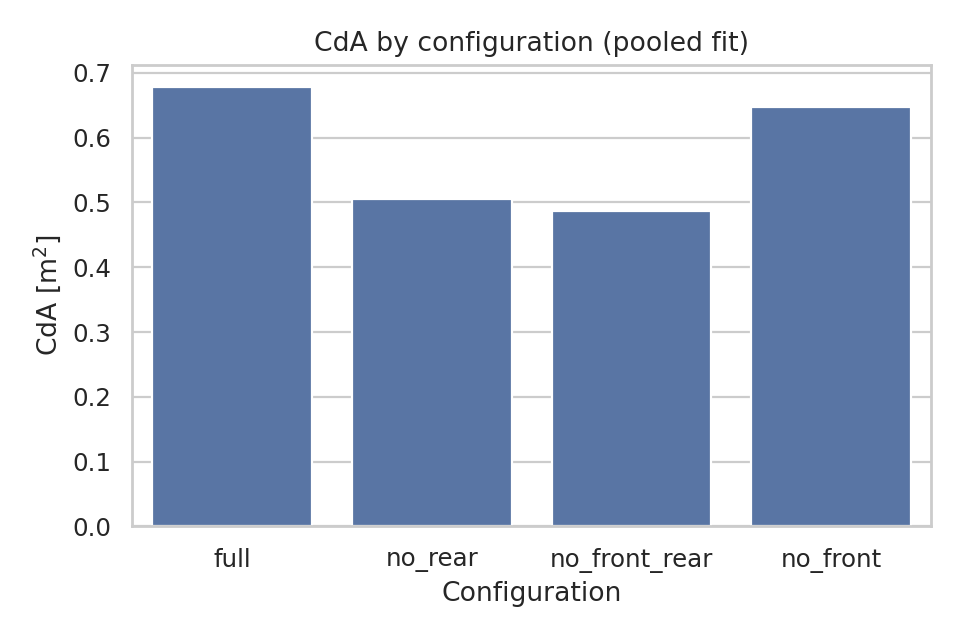
\includegraphics[width=0.85\linewidth]{../../Outputs/03_Drag_Calculation/Approach3_PooledByConfig/plots/CdA_bar_by_config_pooled.png}
  \caption{Approach 3: pooled \(C_dA\) estimate per configuration.}
\end{figure}

\section{Outputs}
Each approach writes:
\begin{itemize}
  \item \texttt{Outputs/03\_Drag\_Calculation/<Approach>/csv/}:
    coefficients, per-config summaries, contributions, and a drag-force table.
  \item \texttt{Outputs/03\_Drag\_Calculation/<Approach>/plots/}:
    summary plots, and (for per-run modes) per-run coastdown fit plots.
\end{itemize}

\section{Results}
This section summarizes the results currently present in
\texttt{Outputs/03\_Drag\_Calculation/}.

\subsection{Uncertainty definition}
The results tables below report measurement uncertainty per configuration:
\begin{itemize}
  \item \textbf{Approach 1}: standard deviation across runs
        (\texttt{CdA\_m2\_std}, \texttt{Cr\_std} from
        \texttt{drag\_config\_summary.csv}).
  \item \textbf{Approach 2}: standard deviation across paired runs.
  \item \textbf{Approach 3}: bootstrap standard deviation of the mean across
        runs.  The bootstrap resamples the per-run $C_dA$ and $C_r$ values
        (from Approach~1) with replacement for $n=300$ iterations (seed~$=1$)
        and reports the standard deviation of the bootstrap means.  Output is
        written to \texttt{bootstrap\_pooled\_uncertainty.csv}.
\end{itemize}

\subsection{Baseline model results (Approaches 1--3)}
Table~\ref{tab:results} summarizes the $C_dA$, $C_r$, and wing-contribution
estimates across all three approaches.

% AUTO-GENERATED FILE. DO NOT EDIT MANUALLY.
% Generated by Docs/scripts/generate_drag_report_tables.py.

% Baseline model results (Approaches 1--3)
\paragraph{Overview: \(C_dA\)}
\begin{table}[h]
\centering
\small
\caption{Baseline model: \(C_dA\) per configuration across Approaches 1--3 (mean/pooled value $\pm$ uncertainty).}
\label{tab:baseline-cda}
\begin{tabular}{lccc}
\toprule
Config & A1 (per-run) & A2 (paired) & A3 (pooled) \\
\midrule
\texttt{full} & $0.661 \pm 0.078$ & $0.661 \pm 0.058$ & $0.679 \pm 0.022$ \\
\texttt{no\_rear} & $0.511 \pm 0.046$ & $0.511 \pm 0.026$ & $0.506 \pm 0.014$ \\
\texttt{no\_front\_rear} & $0.478 \pm 0.057$ & $0.478 \pm 0.048$ & $0.487 \pm 0.015$ \\
\texttt{no\_front} & $0.610 \pm 0.041$ & $0.610 \pm 0.039$ & $0.647 \pm 0.012$ \\
\bottomrule
\end{tabular}
\end{table}

\paragraph{Overview: \(C_r\)}
\begin{table}[h]
\centering
\small
\caption{Baseline model: \(C_r\) per configuration across Approaches 1--3 (mean/pooled value $\pm$ uncertainty).}
\label{tab:baseline-cr}
\begin{tabular}{lccc}
\toprule
Config & A1 (per-run) & A2 (paired) & A3 (pooled) \\
\midrule
\texttt{full} & $0.0235 \pm 0.0043$ & $0.0235 \pm 0.0014$ & $0.0227 \pm 0.0012$ \\
\texttt{no\_rear} & $0.0217 \pm 0.0035$ & $0.0217 \pm 0.0015$ & $0.0217 \pm 0.0009$ \\
\texttt{no\_front\_rear} & $0.0205 \pm 0.0028$ & $0.0205 \pm 0.0013$ & $0.0202 \pm 0.0008$ \\
\texttt{no\_front} & $0.0217 \pm 0.0033$ & $0.0217 \pm 0.0011$ & $0.0201 \pm 0.0010$ \\
\bottomrule
\end{tabular}
\end{table}


\section{Error handling \& robustness}
\begin{itemize}
  \item \textbf{Insufficient data}: if a run slice has fewer than 10 valid
        points after filtering, \texttt{robust\_linear\_fit} raises a
        \texttt{ValueError} and the run is skipped.
  \item \textbf{Negative $R^2$}: reported as-is; indicates the fit is worse than
        a constant model (possible if deceleration is near-constant across the
        speed range, e.g., on a very short run).
  \item \textbf{Empty configuration}: if a config has zero valid runs,
        \texttt{summarize\_by\_config} raises a \texttt{ValueError} when the
        baseline is missing; Approach~3 skips configs with $<50$ pooled samples.
  \item \textbf{Unknown run ID}: runs outside all configured ranges are
        assigned the label \texttt{"unknown"} and excluded from per-config
        summaries.
\end{itemize}

\section{Notes and limitations}
\begin{itemize}
  \item Grade and wind are not explicitly modeled inside a single run; pairing
        opposite directions reduces steady biases if the experiment is designed
        as out-and-back passes.
  \item The $F_{rr}$ force is provided for reference but is constant per
        configuration and does not vary with speed; the primary aerodynamic
        quantity of interest is $C_dA$.
  \item All thresholds (minimum speed, filter gates, bootstrap iterations) can
        be adjusted via CLI arguments of each approach.
\end{itemize}

\end{document}
